\documentclass[12pt]{article}
\usepackage{amsmath}
\usepackage{booktabs}
\usepackage{geometry}
\usepackage{url}
\usepackage[utf8]{inputenc}
\usepackage[T1]{fontenc}
\usepackage{lmodern}
\usepackage{graphicx}

% Für Code-Listings
\usepackage{listings}
\usepackage{xcolor}
\lstset{
  basicstyle=\ttfamily\small,
  keywordstyle=\color{blue},
  commentstyle=\color{gray},
  stringstyle=\color{orange},
  showstringspaces=false,
  frame=single,
  breaklines=true,
  captionpos=b
}

\geometry{a4paper, margin=2.5cm}

\title{Estimating the Number of Legal Chess Diagrams Using Monte Carlo Simulations}
\author{Sven Hans}
\date{October 2025}

\begin{document}
\maketitle

\begin{abstract}
The total number of legal chess diagrams remains unknown due to the immense combinatorial complexity of chess and the difficulty of verifying legality/ reachability. This work presents a Monte Carlo sampling approach that operates on the level of material classes—distinct configurations of chess pieces. For each class, random diagrams are generated and tested for legality using the \texttt{python-chess} library. By combining combinatorial enumeration of diagrams within each class with empirically estimated legal ratios, an overall upper bound for the number of legal chess diagrams without promotions is derived. Our results suggest an upper bound of approximately $7.562\times10^{39}\pm5\%$ legal diagrams, corresponding to roughly one in every 1500 random piece placements being legal. These findings provide a more granular perspective on the distribution of legality across material classes and offer a foundation for future refinements towards even better estimates for upper bounds of legal chess diagrams and chess positions 
\end{abstract}

\section{Introduction and Motivation}

\subsection{Scientific Overview}

Estimating the total number of possible chess diagrams or positions has long been a topic in chess mathematics. Claude Shannon \cite{shannon1950} gave an early rough estimate of the number of possible chess positions. His statement reads:

\begin{quote}
``The number of possible positions, of the general order of 
$64! / (32! \, 8!^2 \, 2!^6)$, or roughly $10^{43}$.''
\end{quote}

This statement originates from Shannon’s foundational 1950 paper. His work focused primarily on the complexity of chess as a game rather than the enumeration of strictly legal positions. 
Modern studies like Chinchalkar 1996 \cite{chinchalkar1996} found an upper bound for the maximum legal chess positions by basic combinatoric and applying restrictions based on chess rules. In 2015 Steinerberger \cite{steinerberger2015} proposed an upper bound for legal diagrams by incorporating the color-lock restriction of bishops. He additionally conjectures that an upper bound of $\approx10^{35}$ for legal diagrams, if one could only incorporate legal pawn structures. Additionally he suggests a Monte Carlo approach to find a tighter upper bound.
2021 Tromp \cite{tromp2021b} implemented a Monte Carlo approach and estimated with 1 Mio samples the upper bound of legal positions (he calls them urpositions) to $\approx10^{44}$. It is not clear to the author, if the approach is restricted to games without promotions or not. 
Due to the immense combinatorial explosion, exact enumeration remains computationally infeasible. Incorporating all chess rules in a combinatoric deduction of the upper count of legal diagrams or positions seems to be too complex to solve. Monte Carlo sampling is currently the most practical approach.

\subsection{Motivation}

Despite decades of research, no exact enumeration of legal chess diagrams or positions exists as of 2025. 
The challenge primarily comes from two aspects: the complex verification of legality 
(ensuring positions obey chess rules such as valid pawn placement, single kings per side, 
castling and en passant rights, and promotions) and reachability 
(ensuring the position can arise from the initial setup by a series of legal moves). 

In addition, many authors apply different restrictions and assumptions when defining or estimating 
the number of chess positions or diagrams. These include whether promotions are allowed, whether illegal pawn 
placements are excluded, or whether only reachable positions are considered. Such differences lead 
to significantly varying numerical estimates. Table~\ref{tab:definitions} summarizes typical definitions 
and includes representative values from the literature.

\begin{table}[h!]
\centering
\renewcommand{\arraystretch}{1.3}
\begin{tabular}{p{3.8cm} p{6.2cm} p{4.9cm}}
\toprule
\textbf{Definition} & \textbf{Description} & \textbf{Upper bounds} \\
\midrule
All diagrams & All possible placements of pieces on the board, ignoring any legality constraints. 
& $\sim 10^{43}$ \cite{shannon1950} \\[0.3em]

Legal diagrams & Diagrams satisfying chess rules (e.g., exactly one king per side, no pawns on rank~1 or~8) without promotions 
& $\approx 1,5\times10^{40}$ \cite{steinerberger2015} $\approx 2.9\times10^{39}$ \cite{tromp2021b} $4\times 10^{37}$ \cite{gourion2021} \\[0.3em]

Legal positions & Legal diagrams with additional information including side to move, castling rights and en~passant possibilities. 
& $\approx (1.78\pm0.04)\times10^{46}$ \cite{chinchalkar1996} , $\approx (4.8\pm0.04)\times10^{44}$ \cite{tromp2021b} \\[0.3em]

Reachable positions & Legal positions that can be reached from the initial setup through valid move sequences. 
&  \\[0.3em]

Legal with promotions & Legal positions including all possible promotions (e.g., multiple queens). 
& \\
\bottomrule
\end{tabular}
\caption{Different definitions of chess \textit{diagrams} and \textit{positions} with corresponding approximate estimates from the literature.}
\label{tab:definitions}
\end{table}

In this paper we try a similar approach like Tromp \cite{tromp2021b}, however we will count legal diagrams without promotions, not positions. In contrary to Tromp's work, we will sample multiple sub spaces defined by single material classes with Monte Carlo and not the full space of diagrams at once.


\section{Methods}

\subsection{Material Classes}

We define a \emph{material class} as a set of specific chess pieces. Each material class specifies the number of kings $K$, queens $Q$, rooks $R$, bishops $B$, knights $N$, and pawns $P$ present for white and black.

\subsubsection{Analytical Calculation}

The number of different material classes can be computed as follows: 
For a single side, the total number of possible piece count combinations with no promotions 
(limits: $K = 1, Q \le 1, R \le 2, B \le 2, N \le 2, P \le 8$) is:

\[
\text{num\_combinations} = (K) \cdot (Q + 1) \cdot (R + 1) \cdot (B + 1) \cdot (N + 1) \cdot (P + 1)
\]

\[
1 \cdot (1 + 1) \cdot (2 + 1) \cdot (2 + 1) \cdot (2 + 1) \cdot (8 + 1) = 486
\]

Since white's and black's piece counts are independent, the total number of
combined material classes is:

\[
486^2 = 236{,}196
\]

\subsubsection{Python Implementation}

The following Python code enumerates all material classes, checking piece
count constraints and total pieces:

\begin{lstlisting}[language=Python, caption={Enumeration of all material classes in chess}, label={lst:material-classes}]
import itertools

limits = {"K": 1, "Q": 1, "R": 2, "B": 2, "N": 2, "P": 8}

def all_side_materials() -> List[Dict[str, int]]:
    """Generate all valid material configurations for one side."""
    side_classes = []
    for q in range(limits["Q"] + 1):
        for r in range(limits["R"] + 1):
             for b in range(limits["B"] + 1):
                 for n in range(limits["N"] + 1):
                    for p in range(limits["P"] + 1):
                        side_classes.append(
                            {"K": 1, "Q": q, "R": r, "B": b, "N": n, "P": p}
                         )
    return side_classes

white_materials = all_side_materials()
black_materials = white_materials.copy()

classes = []
for w, b in itertools.product(white_materials, black_materials):
    total = sum(w.values()) + sum(b.values())
    # Limit total pieces on board
    if total <= 32 and len(w.values()) <=16 and len(b.values()) <= 16:
         classes.append((w, b))
        # Stop early if max_classes reached
         if max_classes is not None and len(classes) >= max_classes:
             break

return classes  # 236196
\end{lstlisting}

\noindent
\textbf{Note:} The check for total pieces per side $\leq 16$ (half the board) and total
pieces $\leq 32$ have been added for enhanced correctness. They are only necessary when including pawn promotions.

\begin{figure}[h!]
  \centering
  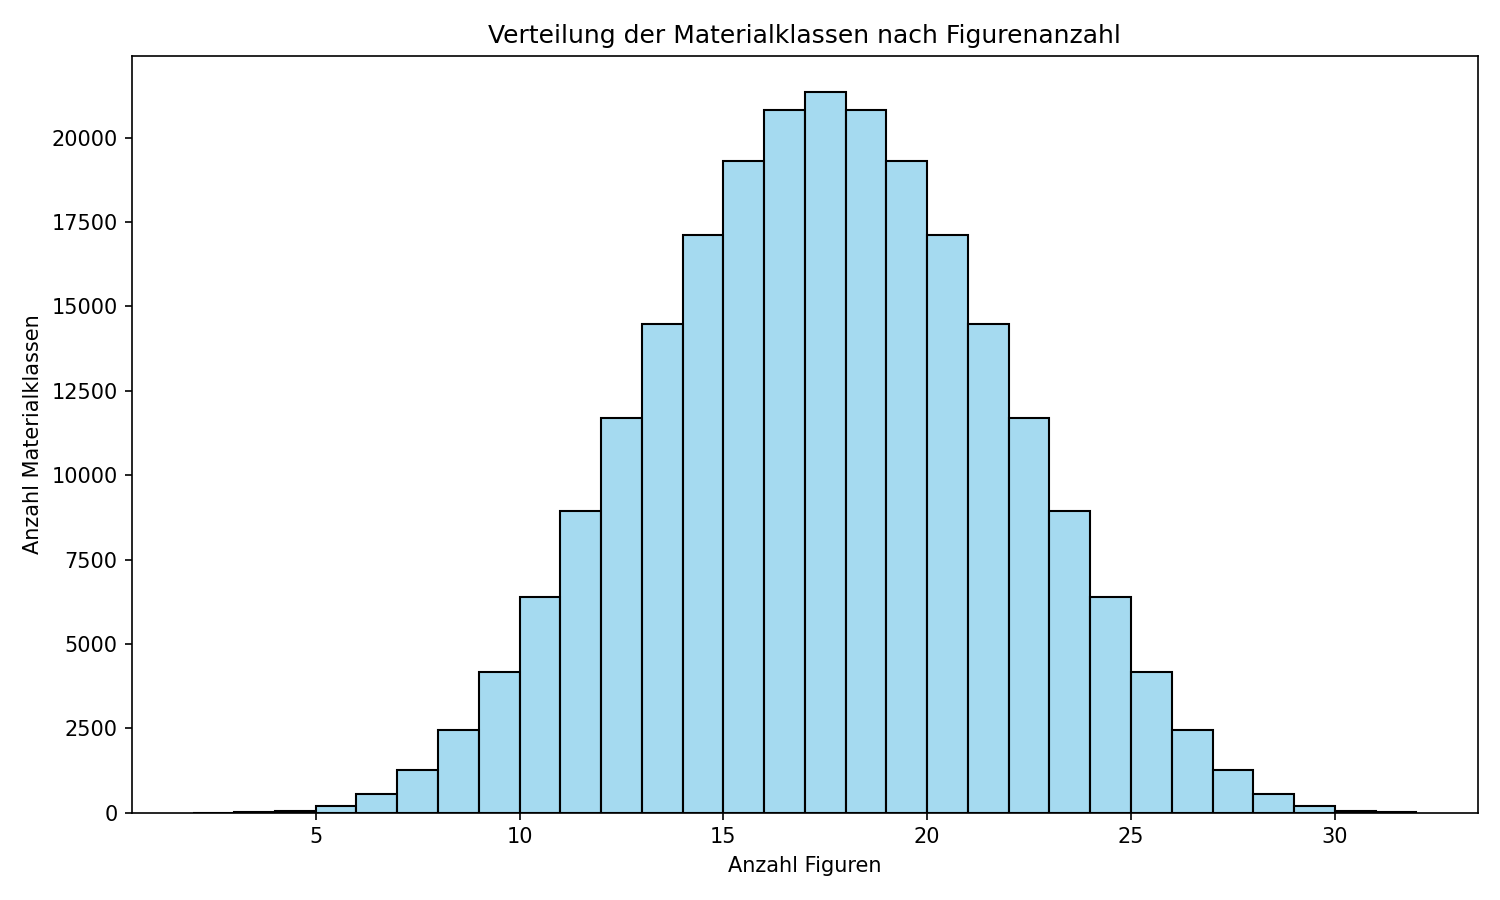
\includegraphics[width=0.8\textwidth]{material_class_histogram.png}
  \caption{Distribution of the count of different material classes for chess pieces count of 2-32}
  \label{fig:material_class_hist}
\end{figure}
Figure \ref{fig:material_class_hist} shows the distribution of different material classes over the number of chess pieces.
\subsection{Diagram Enumeration Within a Material Class}

The total number of ways to distribute the given pieces of a material class over 64 squares (ignoring legality) can be expressed combinatorially as:

\[
\text{Diagrams} = \frac{64!}{(64 - n_w - n_b)! \cdot \prod_i c_i!}
\]

where:
\begin{itemize}
\item $n_w$ and $n_b$ denote the number of white and black pieces, respectively,
\item $c_i$ denotes the count of identical pieces (e.g., two white rooks, eight black pawns).
\end{itemize}

\paragraph{Combinatorial Derivation.}
Let \(n\) denote the total number of pieces to be placed on the 64 squares of the chessboard.  
If all pieces were distinguishable (e.g., labeled), the number of possible placements would correspond to the number of injective mappings from an \(n\)-set to the 64 squares:
\[
64 \cdot 63 \cdot 62 \cdots (64 - n + 1) = \frac{64!}{(64 - n)!}.
\]

In practice, however, many pieces are identical (e.g., the eight white pawns or two black rooks).  
Let \(c_i\) denote the count of identical pieces of type \(i\).  
Since permutations among identical pieces do not yield distinct arrangements, we must divide by the product of the corresponding factorials.  
Thus, the total number of distinct arrangements (ignoring legality) is:
\[
\text{Positions} = \frac{64!}{(64 - n)! \, \prod_i c_i!}.
\]

This formula counts purely geometric placements of the given pieces—commonly referred to as \emph{diagrams}—and ignores all legality constraints (e.g., pawns on the first or eighth rank, both kings in check, etc.).

\paragraph{Example.}
White: 1 King, 1 Queen, 3 Pawns (\(n_w = 5\)) \\
Black: 1 King, 2 Rooks (\(n_b = 3\)) \\
Total \(n = 8\).  
The factorials for identical pieces are \(1!, 1!, 3!, 1!, 2!\).  
Hence:
\[
\text{Positions} = \frac{64!}{(64 - 8)! \, 1! \, 1! \, 3! \, 1! \, 2!}
= \frac{64!}{56! \cdot 3! \cdot 2!}
= 14{,}871{,}915{,}636{,}480 \approx 1.49 \times 10^{13}.
\]

\noindent
\textbf{Note:}  
This formula counts only board \emph{diagrams}.  
A full \emph{position} in chess additionally includes meta-information such as the side to move, castling rights, and possible en-passant targets.  
Therefore, the total number of possible positions is higher, depending on the material configuration.  
Moreover, further constraints must be applied to filter only \emph{legal} positions (e.g., valid king placement, pawn locations, and consistency of castling and check states).

\subsubsection{Legal Diagram Verification Using \texttt{python-chess}}

We employ the \texttt{python-chess} library~\cite{python-chess} to validate generated chess diagrams, ensuring that they satisfy all basic structural legality conditions. 
The library provides a comprehensive set of status flags to detect inconsistencies or impossible states in a given position. 
Among others, the following criteria are verified automatically:

\begin{itemize}
    \item Exactly one king per side (no missing or duplicate kings)
    \item No pawns on the first or last rank
    \item Valid castling rights
    \item Valid en passant squares and consistency with pawn structure
    \item No king in check if it is that side’s turn
    \item No more than two simultaneous checks (\texttt{STATUS\_TOO\_MANY\_CHECKERS})
    \item No geometrically impossible double checks (\texttt{STATUS\_IMPOSSIBLE\_CHECK}), 
          e.g., two attacking pieces aligned on the same ray with the king,
          or en passant positions that cannot have arisen from any legal move
\end{itemize}

\noindent
If none of these error conditions are triggered, the position is marked as 
\texttt{STATUS\_VALID}, meaning it satisfies the fundamental requirements of internal consistency.
However, this does \emph{not} guarantee that the diagram is reachable by a legal sequence of moves from the initial position---it merely ensures that it respects the structural rules of chess.

\begin{lstlisting}[language=Python, caption={Validation of chess positions using python-chess}, label={lst:is_legal}]
import chess

def is_position_legal(board: chess.Board, no_promotion: bool = True) -> bool:
    """
    Check if a random position is legal according to chess rules.

    Args:
        board (chess.Board): The board to check.
        no_promotion (bool): If True, bishop color diversity is enforced.

    Returns:
        bool: True if the position is legal, False otherwise.
    """
    # Basic validity check
    if not board.is_valid():
        return False

    # Pawn column check: no more than 4 pawns in any file per color
    for color in [chess.WHITE, chess.BLACK]:
        pawns_by_file = [0] * 8
        for square in board.pieces(chess.PAWN, color):
            file_idx = chess.square_file(square)
            pawns_by_file[file_idx] += 1
        if any(count >= 5 for count in pawns_by_file):
            return False

    # Bishop color check (only if no_promotion=True)
    if no_promotion:
        for color in [chess.WHITE, chess.BLACK]:
            bishops = list(board.pieces(chess.BISHOP, color))
            if len(bishops) >= 2:
                colors = [((chess.square_file(b) + chess.square_rank(b)) % 2 == 0) for b in bishops]
                if all(colors) or not any(colors):
                    return False

    return True
\end{lstlisting}

\paragraph{Bishop Color Rule.}
The default \texttt{python-chess} legality checks do not enforce the constraint that two bishops of the same color on a side are only possible through pawn promotion. 
To address this, our implementation (see Listing~\ref{lst:is_legal}) adds an explicit bishop color diversity check whenever the \texttt{no\_promotion} flag is enabled. 
This guarantees that each side may have at most one bishop on each color complex, which reflects the structure of a standard chess game without promotions. 
The heuristic ensures that diagrams with ``illegal twin bishops'' on the same color are excluded from the dataset.

\paragraph{Pawn File Rule.}
A further extension of the validation routine concerns pawn distribution across files. 
Our function explicitly rejects any diagram containing five or more pawns of the same color on a single file. 
The reasoning is straightforward: each file has only eight ranks, and pawns cannot pass each other without capturing. 
Since at most two pawns of the same color can coexist in one file (a promoted pawn frees its original square, but new pawns cannot be created), the appearance of five or more pawns is structurally impossible. 
By applying this heuristic, we ensure that positions remain consistent with the basic combinatorial constraints of chess pawn structure.

\subsection{Monte Carlo Sampling and Legal Ratio Estimation}

For each material class, we estimate the fraction of legal diagrams by Monte Carlo sampling. Random diagrams are generated by placing the pieces of the class uniformly at random on the $64$ squares, and each diagram is tested for legality using the \texttt{python-chess} library (see Section~2.2.1).

Let $n$ denote the number of sampled diagrams and $l$ the number among them that pass the legality check. The legal ratio for the material class is then estimated as
\begin{equation}
\hat{r} \;=\; \frac{l}{n}\, .
\end{equation}

\subsubsection{Adaptive Sample Size Determination}

To obtain stable estimates without oversampling easy classes, we use an adaptive sampling scheme that increases the sample size only as needed. The procedure implemented in our code is:

\begin{enumerate}
  \item \textbf{Initialization.} Start with a baseline sample size $n_0 \in \{1000, 2000\}$ and draw $n_0$ random diagrams for the class. Record the number $l_0$ of legal diagrams and compute the initial estimate $\hat{r}_0 = l_0/n_0$.
  \item \textbf{Incremental refinement (accumulating samples).} If more precision is required, we \emph{do not} discard previous samples. Instead, we double the target sample size $n \leftarrow \min(2n,\,128{,}000)$ and draw only the \emph{additional} diagrams needed to reach $n$. Let $k$ be the cumulative number of legal diagrams out of the cumulative $n$ samples; update $\hat{r}=k/n$.
  \item \textbf{Error estimation per iteration.} After each update we compute the binomial standard error
  \begin{equation}
     \mathrm{SE}(\hat{r}) \;=\; \sqrt{\frac{\hat{r}(1-\hat{r})}{n}}\, ,
  \end{equation}
  and its relative form $\mathrm{rSE}(\hat{r}) = \mathrm{SE}(\hat{r})/\hat{r}$ (defined as $1$ if $\hat{r}=0$).
  \item \textbf{Stopping rule.} We stop when the relative standard error is below the threshold
  \begin{equation}
     \frac{\mathrm{SE}(\hat{r})}{\hat{r}} \;<\; 0.10,
  \end{equation}
  or when the cap $n \le 128{,}000$ is reached. Thus, per-class relative uncertainty is \emph{at most} $10\%$ by construction, and often substantially smaller.
\end{enumerate}

This adaptive, cumulative design concentrates computation on difficult classes (small $\hat{r}$ or high variance), while simple classes terminate early.

\subsubsection{Statistical Properties and Error Propagation}

Assuming independence between classes, the total number of legal diagrams is estimated as
\begin{equation}
\hat{N}_{\text{legal}} \;=\; \sum_{i} d_i\,\hat{r}_i \,,
\end{equation}
where $d_i$ is the (theoretical) diagram count of class $i$ and $\hat{r}_i$ its estimated legal ratio. For each class $i$, the binomial standard error is
\[
\mathrm{SE}(\hat{r}_i) \;=\; \sqrt{\frac{\hat{r}_i(1-\hat{r}_i)}{n_i}} \, .
\]
By linear error propagation, the variance of the global estimate is
\begin{equation}
\mathrm{Var}\!\left(\hat{N}_{\text{legal}}\right) \;=\; \sum_i d_i^2\,\mathrm{SE}(\hat{r}_i)^2
\quad\Rightarrow\quad
\mathrm{SE}\!\left(\hat{N}_{\text{legal}}\right) \;=\; 
\sqrt{ \sum_i d_i^2\,\mathrm{SE}(\hat{r}_i)^2 } \, .
\end{equation}
A convenient global relative uncertainty is then
\begin{equation}
\mathrm{rSE}\!\left(\hat{N}_{\text{legal}}\right)
\;=\;
\frac{\mathrm{SE}\!\left(\hat{N}_{\text{legal}}\right)}{\hat{N}_{\text{legal}}}\, .
\end{equation}

\paragraph{Observed precision.}
Because each class is sampled until its \emph{per-class} relative standard error is at most $10\%$, the final per-class uncertainties lie at or below this threshold (many classes finish below it). Aggregating across all material classes with the variance formula above, we obtained a \emph{global} relative standard error of approximately \textbf{4.1\%} for $\hat{N}_{\text{legal}}$, reflecting averaging across a very large number of independent class estimates.

\section{Results}

Based on the Monte Carlo sampling approach described above, the total number of \emph{legal chess diagrams} (i.e., piece arrangements satisfying the structural rules of chess but not necessarily reachable by legal play) was estimated.

For each material class $m$, the total number of diagrams was computed combinatorially, and multiplied by the empirically estimated \emph{valid ratio}~$r_m$ obtained from the Monte Carlo simulations.  
The overall estimate across all material classes is therefore given by:

\[
N_{\text{legal}} = \sum_{m \in \mathcal{M}} r_m \cdot N_m,
\]

where:
\begin{itemize}
    \item $\mathcal{M}$ denotes the set of all material classes (possible distributions of pieces by type and color),
    \item $N_m$ is the total number of diagrams for material class~$m$,
    \item $r_m$ is the fraction of those diagrams that are structurally legal according to \texttt{python-chess}.
\end{itemize}

Using this procedure, the estimated upper bound for the total number of legal diagrams is:

\[
N_{\text{legal}} \approx 7.562 \times 10^{39}\pm3.1^{38} (4.1\%).
\]
To compute this bound we did calculate about 4000 samples per material class (median) and checked the legality: In total about $3\times 10^{9}$ sample diagrams. The minimum sample size was 1000 for some classes and the maximum 128000 for others. As stated above we used a sampling method with adaptive sizes per material class.
\noindent
When compared to the total number of all possible diagrams (i.e., all unconstrained piece placements across all material classes), the global ratio of legal to total diagrams was found to be approximately:

\[
\frac{N_{\text{legal}}}{N_{\text{all}}} \approx 6.376 \times 10^{-4}.
\]

This indicates that fewer than one in every 1500 random piece configurations satisfies even the basic structural rules of chess, stated above.
The valid ratio~$r_m$ is, however, \emph{not constant} across material classes: positions with a small number of pieces (e.g., king and pawns only) or heavily asymmetrical material distributions exhibit a higher probability of structural legality, while classes with many pieces or numerous pawns show significantly lower ratios due to increased likelihood of overlapping or invalid pawn placements.

These results represent an upper bound, as the legality checks performed do not include color-complex restrictions for bishops or reachability constraints based on move sequences. The legality check does also not include unreachable pawn patterns, like more than 4 pawns in one column or unreachable side-pawn patterns \cite{mcdonagh2022}.

\begin{figure}[h!]
  \centering
  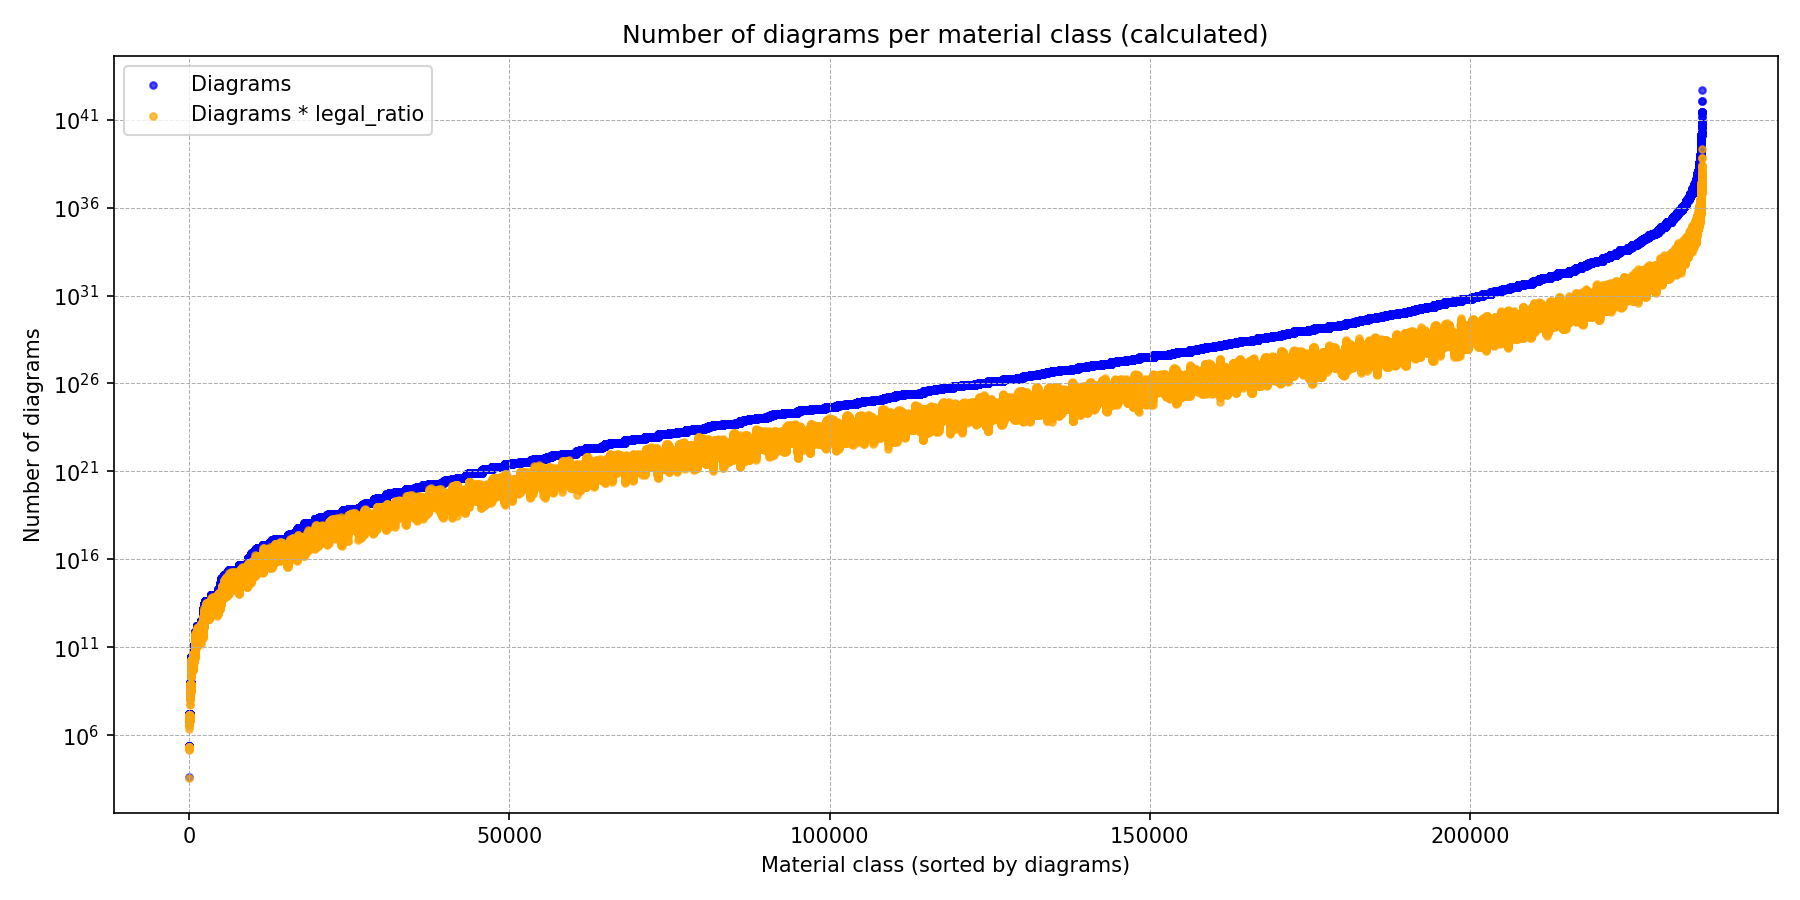
\includegraphics[width=0.8\textwidth]{diagrams_per_class.png}
  \caption{Count of diagrams and legal diagrams over the rank of each material class. The rank of a classes is defined by sorting by the number of all diagrams of the classes.}
  \label{fig:diagrams_per_class}
\end{figure}
In \ref{fig:diagrams_per_class} one may observe, that only very few of material classes have a huge impact on the total number of possible (legal) diagrams. Therefore it would be sufficient to only analyze these classes to come up with a good approximation of the stated upper bound for legal diagrams. The noise in the legal diagrams line, is probably due to the statistical approach and an insufficient sample size. However, we also expect a variation as the true legal ratio may fluctuate between material classes with adjacent rank.

\begin{figure}[h!]
  \centering
  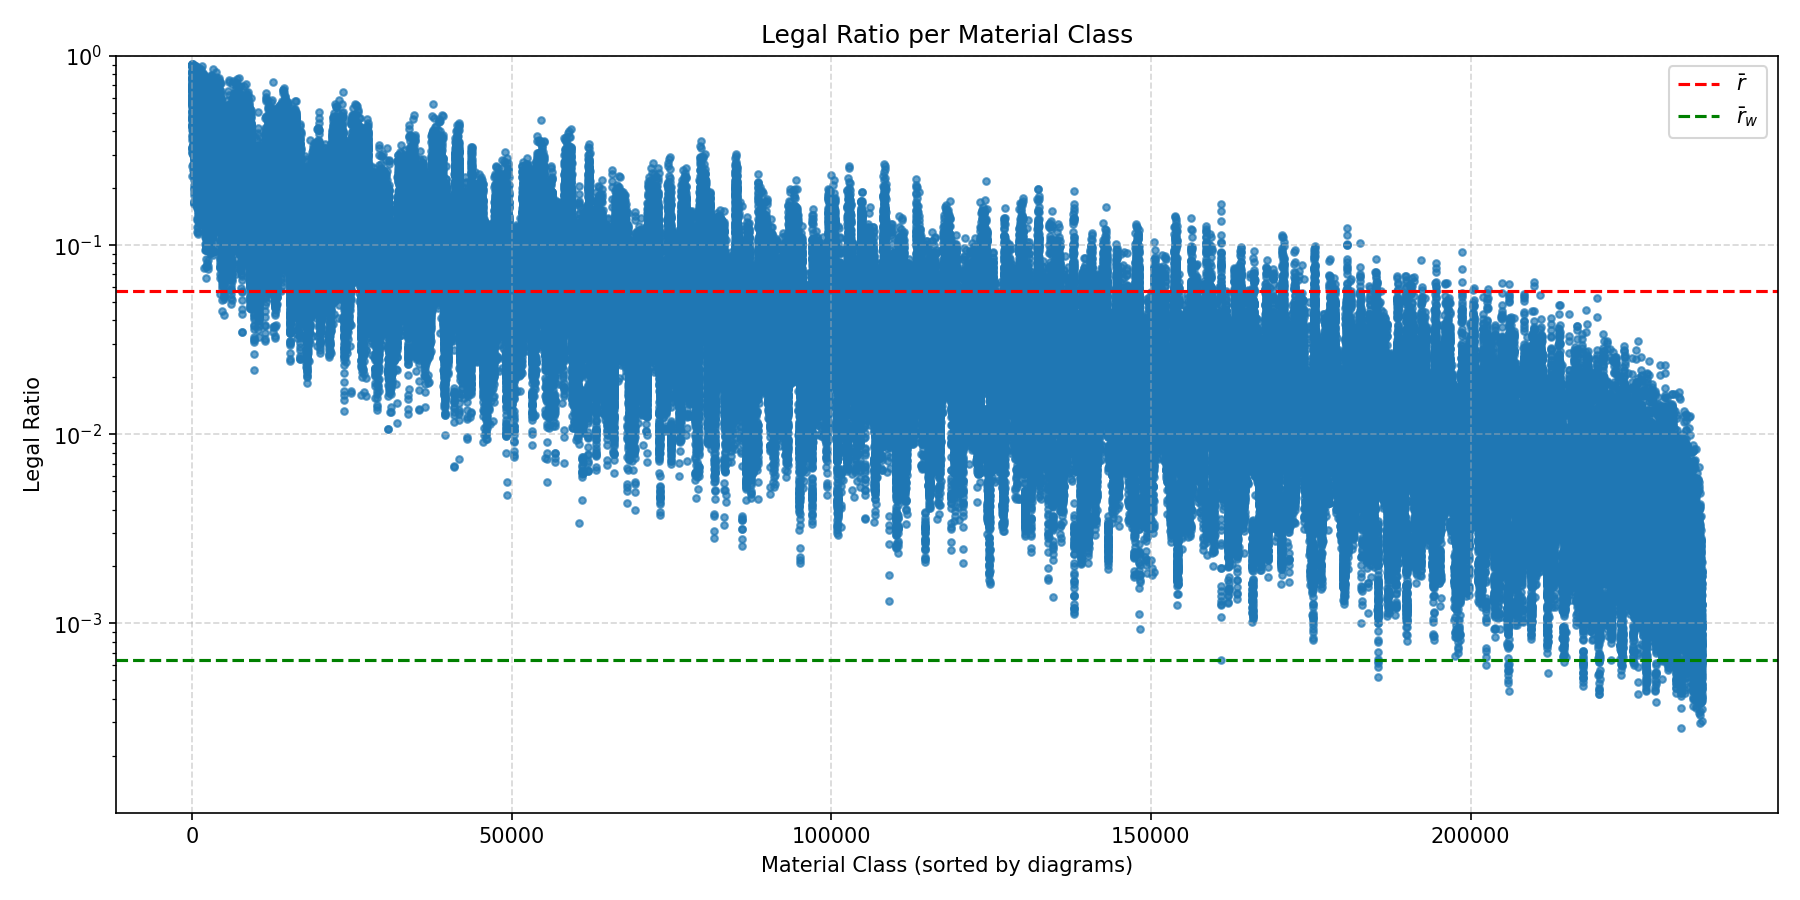
\includegraphics[width=0.8\textwidth]{legal_ratio_per_class.png}
  \caption{Legal ratio over the rank of material classes.}
  \label{fig:legal_ratio_by_class}
\end{figure}

The figure \ref{fig:diagrams_per_class} shows the legal ratio over all classes, with classes sorted in the same way, as in figure \ref{fig:diagrams_per_class}. One may observe a noisy variation of the legal ratio in dependence of the material class. There is also a systematic drift, with low ratio for classes with high rank. Meaning the fraction of illegal diagrams is higher for classes with large counts of different diagrams.


\begin{figure}[h!]
  \centering
  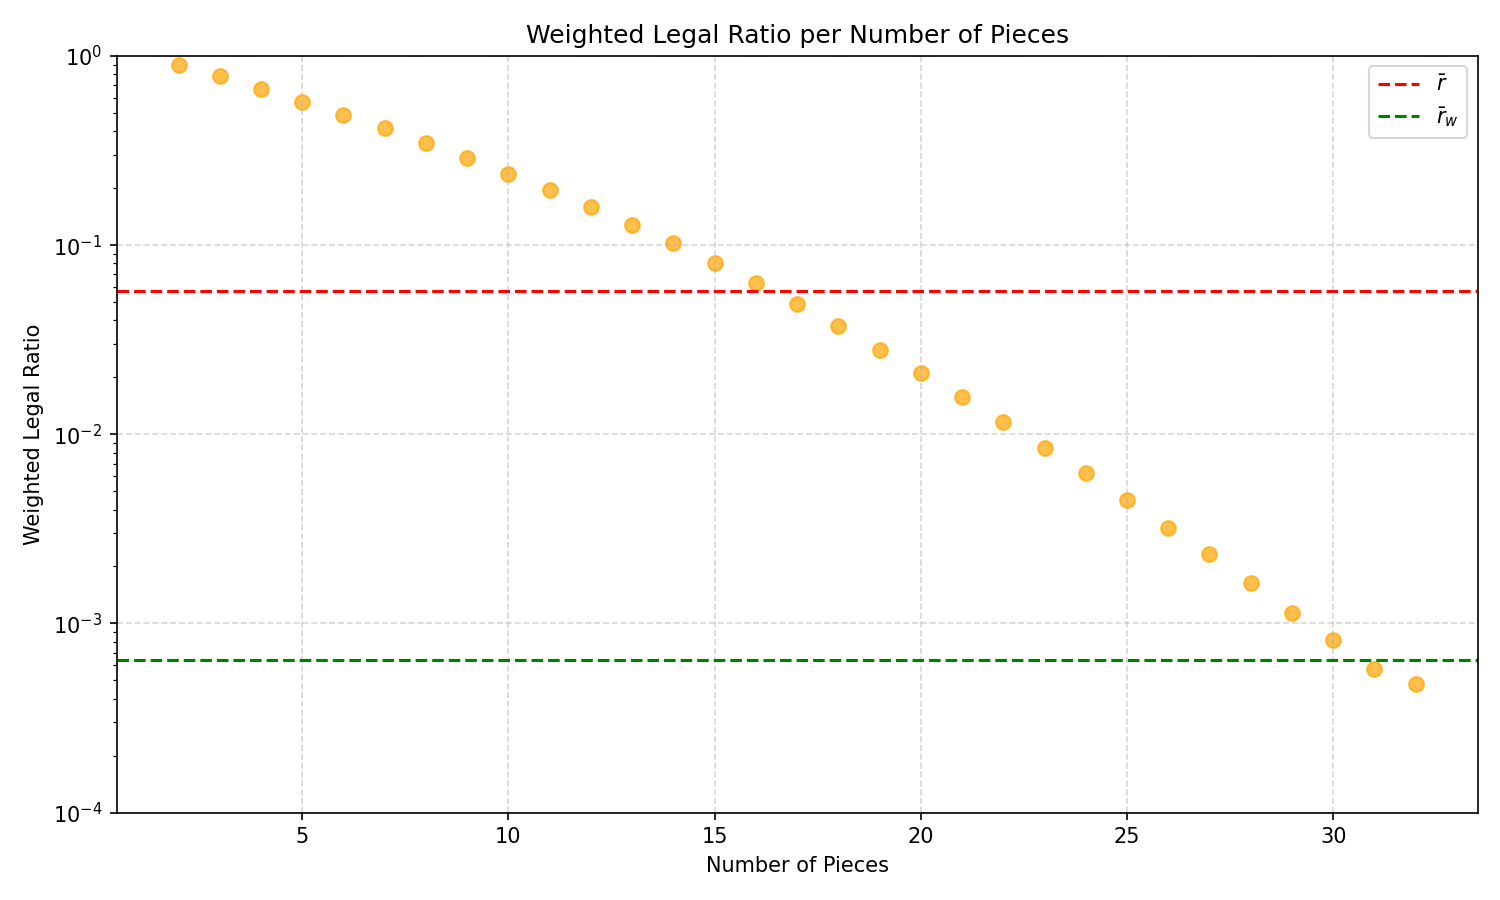
\includegraphics[width=0.8\textwidth]{legal_ratio_per_num_pieces.png}
  \caption{Average Legal ratio over number of chess pieces}
  \label{fig:legal_ratio_by_pieces}
\end{figure}
Figure \ref{fig:legal_ratio_by_pieces} shows the average legal ratio over the number of chess pieces. One observes, that the lowest fraction of legal diagrams can be found for 32 pieces. This indicates again, that for solving the problem of finding an upper bound for legal diagrams or positions, analyzing games with high number of pieces is most important.
\begin{figure}[h!]
  \centering
  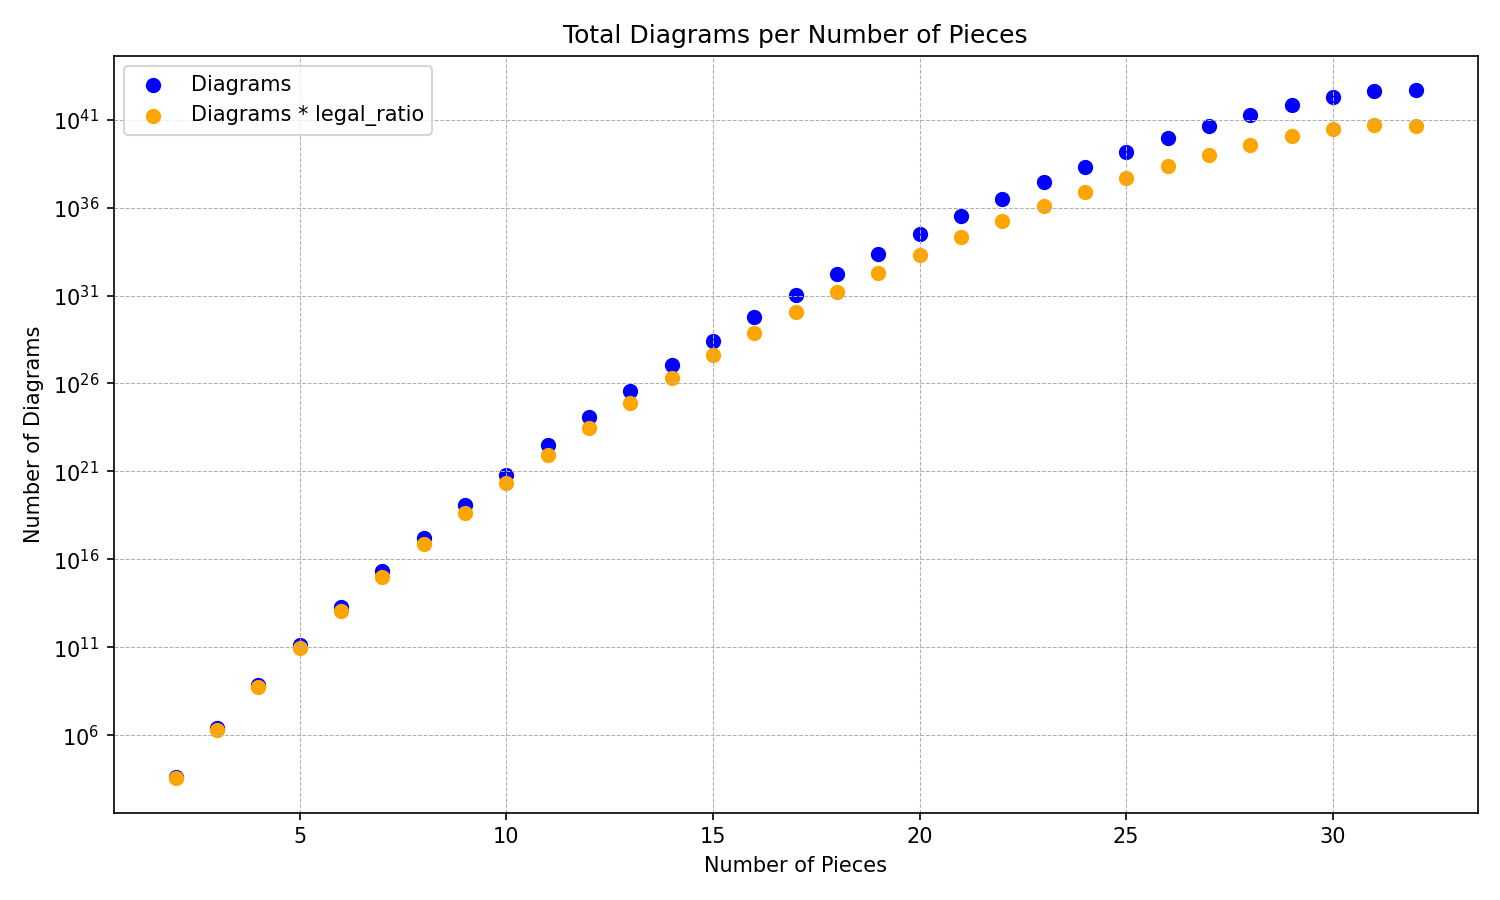
\includegraphics[width=0.8\textwidth]{diagrams_per_num_pieces.png}
  \caption{Average (legal) diagrams over number of chess pieces}
  \label{fig:diagrams_by_pieces}
\end{figure}

Finally figure \ref{fig:diagrams_by_pieces} shows the number of total and legal diagrams over the number of chess pieces. Interestingly we find the maximum of legal diagrams for 31 pieces and not 32, like for the total number of diagrams.

\section{Summary and Conclusion}

This study demonstrates that Monte Carlo simulations can provide meaningful statistical estimates for the otherwise intractable problem of enumerating legal chess diagrams. By decomposing the search space into well-defined material classes and applying legality checks on sampled diagrams, we approximate the total number of structurally valid configurations to be on the order of $10^{40}$.

The data reveal strong variations in the legality ratio across material classes and a systematic decline for positions with a high total number of pieces, especially near the full 32-piece configuration. This indicates that illegalities such as invalid pawn placements and conflicting king states dominate in dense positions.

Our findings also highlight that only a small subset of material classes significantly contributes to the global count — primarily those with near-complete sets of pieces. This observation suggests a strategy for future refinements: focus computational effort on high-impact material classes while applying statistical interpolation for the rest.

While this work excludes promotions and reachability constraints, it provides a scalable foundation for estimating the space of \emph{legal} (but not necessarily \emph{reachable}) chess diagrams. Extending the method to include promoted pieces, bishop color and pawn structure constraints represents a promising direction for further research.

\section{References}

\begin{thebibliography}{9}

\bibitem{shannon1950}
C. E. Shannon, \emph{Programming a Computer for Playing Chess}, 
\textit{Philosophical Magazine}, Vol.~41, pp.~256–275, 1950.

\bibitem{chinchalkar1996}
S.,S. Chinchalkar, \emph{An Upper Bound for the Number of Reachable Positions},
\textit{ICCA Journal}, Vol. 19, No. 3 (Sept. 1996), pp. 181–183. DOI:10.3233/ICG-1996-19305.

\bibitem{steinerberger2015}
S.,Steinerberger, \emph{On the number of positions in chess without promotion},
\textit{International Journal of Game Theory}, Vol.,44, No.,3 (Aug. 2015), pp.,761-767. DOI:10.1007/s00182-014-0453-7. 

\bibitem{tromp2021b}
J. Tromp, \emph{Chess Position Ranking}, GitHub repository, Dec.~2021. 
\url{https://github.com/tromp/ChessPositionRanking}

\bibitem{python-chess}
N. Fiekas, “python-chess: A Chess Library for Python,” 
\url{https://python-chess.readthedocs.io/}

\bibitem{gourion2021}
D. Gourion, \emph{An Upper Bound for the Number of Chess Diagrams Without Promotion}, 
arXiv preprint \textit{arXiv:2112.09386}, 2021.

\bibitem{mcdonagh2022}
C. McDonagh, \emph{Counting Unreachable Single-Side Pawn Diagrams with Limitless Captures}, 
\textit{arXiv preprint} arXiv:2202.00428v1, 2022.

\end{thebibliography}

\end{document}
